\documentclass[a4paper, 12pt]{article}
\usepackage{xeCJK}
    \setCJKmainfont[AutoFakeBold=1,AutoFakeSlant=.4]{標楷體}
    \XeTeXlinebreaklocale "zh"
    \XeTeXlinebreakskip = 0pt plus 1pt
\usepackage{fontspec}
    \setmainfont{Times New Roman}
\usepackage{setspace}
    \onehalfspace
    \setlength{\parskip}{1ex plus 0.5ex minus 0.2ex}
\usepackage{mathtools}
\usepackage{graphicx}
\usepackage{enumitem}
\parindent=0pt
\def\Large{\fontsize{16}{24}\selectfont}
\def\large{\fontsize{14}{20}\selectfont}
\makeatletter
\renewcommand\section{\@startsection {section}{1}{\z@}%
                                   {-3.5ex \@plus -1ex \@minus -.2ex}%
                                   {2.3ex \@plus.2ex}%
                                   {\centering\normalfont\Large\bfseries}}
\renewcommand\subsection{\@startsection {subsection}{1}{\z@}%
                                   {-3.5ex \@plus -1ex \@minus -.2ex}%
                                   {2.3ex \@plus.2ex}%
                                   {\centering\normalfont\large\bfseries}}
\makeatother
\begin{document}

\section*{CO ,lag and moving average data}
smooth terms P-value
\begin{table}[ht]
\centering
\begin{tabular}{rrrrrrrr}
  \hline
 & s.pv & mv2 & mv3 & mv4 & mv5 & mv6 & mv7 \\
  \hline
1 & 0.0008 & 0.0006 & 0.1193 & 0.0623 & 0.0000 & 0.0009 & 0.0005 \\
  2 & 0.0014 & 0.0030 & 0.0265 & 0.0433 & 0.2549 & 0.0201 & 0.0010 \\
  3 & 0.0000 & 0.0000 & 0.0089 & 0.0000 & 0.0088 & 0.0056 & 0.0071 \\
  4 & 0.0000 & 0.3721 & 0.0037 & 0.0000 & 0.0001 & 0.0002 & 0.0006 \\
  5 & 0.5043 & 0.1307 & 0.0088 & 0.2186 & 0.0026 & 0.0148 & 0.0000 \\
  6 & 0.0004 & 0.0134 & 0.0072 & 0.1784 & 0.0023 & 0.0025 & 0.0000 \\
  7 & 0.0000 & 0.0000 & 0.0916 & 0.0002 & 0.0245 & 0.0001 & 0.0000 \\
  8 & 0.0000 & 0.0000 & 0.2019 & 0.0016 & 0.5944 & 0.3357 & 0.1483 \\
   \hline
\end{tabular}
\end{table}
\clearpage
\section*{SO2,lag and moving average data}
smooth terms P-value
\begin{table}[ht]
\centering
\begin{tabular}{rrrrrrrr}
  \hline
 & s.pv & mv2 & mv3 & mv4 & mv5 & mv6 & mv7 \\
  \hline
1 & 0.0031 & 0.0000 & 0.0202 & 0.0007 & 0.0000 & 0.0004 & 0.0007 \\
  2 & 0.0208 & 0.0013 & 0.0001 & 0.0103 & 0.0002 & 0.0020 & 0.0002 \\
  3 & 0.0000 & 0.0044 & 0.2513 & 0.0006 & 0.0042 & 0.0306 & 0.0046 \\
  4 & 0.0019 & 0.0091 & 0.0307 & 0.0966 & 0.0843 & 0.0315 & 0.0080 \\
  5 & 0.0000 & 0.0232 & 0.1186 & 0.5243 & 0.2252 & 0.1371 & 0.0033 \\
  6 & 0.4750 & 0.0009 & 0.2361 & 0.1678 & 0.0472 & 0.0245 & 0.0065 \\
  7 & 0.0019 & 0.0009 & 0.1396 & 0.0000 & 0.0004 & 0.0005 & 0.2161 \\
  8 & 0.2093 & 0.0033 & 0.4614 & 0.0000 & 0.0041 & 0.0494 & 0.0012 \\
   \hline
\end{tabular}
\end{table}
\clearpage
\section*{O3,lag and moving average data}
smooth terms P-value
\begin{table}[ht]
\centering
\begin{tabular}{rrrrrrrr}
  \hline
 & s.pv & mv2 & mv3 & mv4 & mv5 & mv6 & mv7 \\
  \hline
1 & 0.0029 & 0.0000 & 0.0159 & 0.0018 & 0.0067 & 0.0017 & 0.0281 \\
  2 & 0.0010 & 0.0001 & 0.0064 & 0.0011 & 0.0136 & 0.0031 & 0.0311 \\
  3 & 0.0001 & 0.0519 & 0.0649 & 0.0016 & 0.0536 & 0.0113 & 0.0523 \\
  4 & 0.0005 & 0.0292 & 0.0036 & 0.0145 & 0.0165 & 0.0161 & 0.0112 \\
  5 & 0.0156 & 0.0020 & 0.2877 & 0.0127 & 0.2071 & 0.0002 & 0.0037 \\
  6 & 0.0437 & 0.0000 & 0.1755 & 0.0061 & 0.0353 & 0.0000 & 0.1791 \\
  7 & 0.0003 & 0.0297 & 0.2335 & 0.0027 & 0.0842 & 0.0817 & 0.0171 \\
  8 & 0.0023 & 0.0054 & 0.0247 & 0.1438 & 0.1641 & 0.5457 & 0.0184 \\
   \hline
\end{tabular}
\end{table}
\clearpage
\section*{PM2.5 ,lag and moving average data}
smooth terms P-value
\begin{table}[ht]
\centering
\begin{tabular}{rrrrrrrr}
  \hline
 & s.pv & mv2 & mv3 & mv4 & mv5 & mv6 & mv7 \\
  \hline
1 & 0.0005 & 0.0722 & 0.0000 & 0.0328 & 0.0105 & 0.0001 & 0.0002 \\
  2 & 0.0006 & 0.0098 & 0.0024 & 0.0000 & 0.0027 & 0.0013 & 0.0001 \\
  3 & 0.0296 & 0.0012 & 0.0000 & 0.0287 & 0.0000 & 0.0000 & 0.0000 \\
  4 & 0.0000 & 0.0000 & 0.0000 & 0.0027 & 0.0507 & 0.0042 & 0.0003 \\
  5 & 0.0005 & 0.0361 & 0.0049 & 0.0026 & 0.1241 & 0.1831 & 0.0210 \\
  6 & 0.0021 & 0.0024 & 0.2872 & 0.4540 & 0.0198 & 0.1221 & 0.0068 \\
  7 & 0.0004 & 0.1174 & 0.0008 & 0.0055 & 0.0217 & 0.0630 & 0.6479 \\
  8 & 0.0485 & 0.0013 & 0.3106 & 0.9563 & 0.0197 & 0.2248 & 0.3089 \\
   \hline
\end{tabular}
\end{table}
\clearpage
\section*{ PM10,lag and moving average data}
smooth terms P-value
\begin{table}[ht]
\centering
\begin{tabular}{rrrrrrrr}
  \hline
 & s.pv & mv2 & mv3 & mv4 & mv5 & mv6 & mv7 \\
  \hline
1 & 0.1665 & 0.1394 & 0.1810 & 0.0010 & 0.0018 & 0.0036 & 0.0007 \\
  2 & 0.0000 & 0.0036 & 0.0905 & 0.0033 & 0.0006 & 0.0005 & 0.0001 \\
  3 & 0.0015 & 0.0001 & 0.0000 & 0.0025 & 0.0382 & 0.0038 & 0.0029 \\
  4 & 0.0074 & 0.0082 & 0.0042 & 0.0004 & 0.0027 & 0.0062 & 0.0059 \\
  5 & 0.1604 & 0.0658 & 0.0684 & 0.0214 & 0.0042 & 0.0105 & 0.0200 \\
  6 & 0.0148 & 0.0001 & 0.0004 & 0.1942 & 0.0099 & 0.0003 & 0.0387 \\
  7 & 0.0007 & 0.0219 & 0.1055 & 0.0000 & 0.0017 & 0.0000 & 0.0000 \\
  8 & 0.0343 & 0.8177 & 0.1650 & 0.7408 & 0.0236 & 0.1863 & 0.0560 \\
   \hline
\end{tabular}
\end{table}
\clearpage
\section*{ NO2,lag and moving average data}
smooth terms P-value
\begin{table}[ht]
\centering
\begin{tabular}{rrrrrrrr}
  \hline
 & s.pv & mv2 & mv3 & mv4 & mv5 & mv6 & mv7 \\
  \hline
1 & 0.0004 & 0.0034 & 0.1743 & 0.0088 & 0.0252 & 0.0032 & 0.0008 \\
  2 & 0.0001 & 0.0012 & 0.0001 & 0.0003 & 0.0105 & 0.0014 & 0.0050 \\
  3 & 0.0009 & 0.0000 & 0.0001 & 0.0064 & 0.0274 & 0.0228 & 0.0042 \\
  4 & 0.0001 & 0.0857 & 0.0055 & 0.0532 & 0.0001 & 0.0014 & 0.0092 \\
  5 & 0.0674 & 0.0000 & 0.0000 & 0.0007 & 0.0000 & 0.0013 & 0.0011 \\
  6 & 0.0141 & 0.0418 & 0.0051 & 0.0000 & 0.0006 & 0.0027 & 0.0010 \\
  7 & 0.0000 & 0.0000 & 0.0002 & 0.0001 & 0.0022 & 0.0002 & 0.0017 \\
  8 & 0.1031 & 0.0030 & 0.0012 & 0.3444 & 0.0227 & 0.0472 & 0.0953 \\
   \hline
\end{tabular}
\end{table}
\clearpage
\section*{NO ,lag and moving average data}
smooth terms P-value
\begin{table}[ht]
\centering
\begin{tabular}{rrrrrrrr}
  \hline
 & s.pv & mv2 & mv3 & mv4 & mv5 & mv6 & mv7 \\
  \hline
1 & 0.0096 & 0.0000 & 0.0008 & 0.0000 & 0.0000 & 0.0001 & 0.0008 \\
  2 & 0.0000 & 0.0097 & 0.7004 & 0.0128 & 0.0057 & 0.0000 & 0.0000 \\
  3 & 0.0000 & 0.1035 & 0.0001 & 0.0035 & 0.0034 & 0.0063 & 0.0001 \\
  4 & 0.0014 & 0.0062 & 0.1024 & 0.0006 & 0.0149 & 0.0004 & 0.0002 \\
  5 & 0.0000 & 0.0000 & 0.0759 & 0.0111 & 0.0003 & 0.0337 & 0.0143 \\
  6 & 0.2941 & 0.0014 & 0.0180 & 0.0005 & 0.0756 & 0.0000 & 0.0088 \\
  7 & 0.0000 & 0.1351 & 0.2382 & 0.0001 & 0.0025 & 0.0000 & 0.1229 \\
  8 & 0.0000 & 0.1449 & 0.0028 & 0.3272 & 0.0007 & 0.1495 & 0.0001 \\
   \hline
\end{tabular}
\end{table}
\clearpage
\section*{O3+PM2.5+TEMP+RH ,lag and moving average data}
O3 linear term p-value\\
\begin{table}[ht]
\centering
\begin{tabular}{rrrrrrrr}
  \hline
 & p.pv & mv2 & mv3 & mv4 & mv5 & mv6 & mv7 \\
  \hline
1 & 0.09 & 0.16 & 0.67 & 0.99 & 0.47 & 0.69 & 0.51 \\
  2 & 0.02 & 0.72 & 0.97 & 0.18 & 0.49 & 0.25 & 0.40 \\
  3 & 0.06 & 0.91 & 0.15 & 0.14 & 0.92 & 0.65 & 0.82 \\
  4 & 0.00 & 0.30 & 0.06 & 0.78 & 0.88 & 0.43 & 0.75 \\
  5 & 0.52 & 0.11 & 0.63 & 0.14 & 0.84 & 0.89 & 0.54 \\
  6 & 0.15 & 0.23 & 0.65 & 0.85 & 0.38 & 0.95 & 0.73 \\
  7 & 0.58 & 0.23 & 0.36 & 0.69 & 0.79 & 0.52 & 0.92 \\
  8 & 0.04 & 0.13 & 0.06 & 0.15 & 0.78 & 0.36 & 0.95 \\
   \hline
\end{tabular}
\end{table}
\\
PM2.5 linear term p-value\\
\begin{table}[ht]
\centering
\begin{tabular}{rrrrrrrr}
  \hline
 & p.pv & mv2 & mv3 & mv4 & mv5 & mv6 & mv7 \\
  \hline
1 & 0.00 & 0.00 & 0.62 & 0.09 & 0.74 & 0.44 & 0.42 \\
  2 & 0.00 & 0.63 & 0.59 & 0.23 & 0.80 & 0.33 & 0.74 \\
  3 & 0.00 & 0.41 & 0.00 & 0.01 & 0.39 & 0.08 & 0.69 \\
  4 & 0.14 & 0.20 & 0.26 & 0.30 & 0.22 & 0.88 & 0.31 \\
  5 & 0.96 & 0.30 & 0.34 & 0.21 & 0.54 & 0.49 & 0.83 \\
  6 & 0.95 & 0.90 & 0.26 & 0.66 & 0.17 & 0.88 & 0.63 \\
  7 & 0.52 & 0.45 & 0.87 & 0.45 & 0.59 & 0.24 & 0.91 \\
  8 & 0.09 & 0.16 & 0.14 & 0.41 & 0.98 & 0.26 & 0.64 \\
   \hline
\end{tabular}
\end{table}
\clearpage
temp smooth p-value
\begin{table}[ht]
\centering
\begin{tabular}{rrrrrrrr}
  \hline
 & s.pv & mv2 & mv3 & mv4 & mv5 & mv6 & mv7 \\
  \hline
1 & 0.00 & 0.00 & 0.06 & 0.01 & 0.10 & 0.02 & 0.02 \\
  2 & 0.23 & 0.19 & 0.14 & 0.65 & 0.23 & 0.26 & 0.09 \\
  3 & 0.00 & 0.68 & 0.00 & 0.00 & 0.09 & 0.01 & 0.07 \\
  4 & 0.82 & 0.26 & 0.70 & 0.22 & 0.06 & 0.27 & 0.05 \\
  5 & 0.48 & 0.86 & 0.53 & 0.56 & 0.43 & 0.16 & 0.28 \\
  6 & 0.80 & 0.53 & 0.40 & 0.79 & 0.39 & 0.57 & 0.25 \\
  7 & 0.12 & 0.15 & 0.57 & 0.81 & 0.52 & 0.74 & 0.42 \\
  8 & 0.14 & 0.13 & 0.11 & 0.47 & 0.85 & 0.30 & 0.92 \\
   \hline
\end{tabular}
\end{table}
\\
rh smooth p-value
\begin{table}[ht]
\centering
\begin{tabular}{rrrrrrrr}
  \hline
 & s.pv & mv2 & mv3 & mv4 & mv5 & mv6 & mv7 \\
  \hline
1 & 0.00 & 0.00 & 0.00 & 0.00 & 0.00 & 0.01 & 0.00 \\
  2 & 0.63 & 0.01 & 0.00 & 0.00 & 0.01 & 0.00 & 0.00 \\
  3 & 0.20 & 0.22 & 0.00 & 0.00 & 0.00 & 0.00 & 0.00 \\
  4 & 0.89 & 0.16 & 0.85 & 0.11 & 0.01 & 0.01 & 0.01 \\
  5 & 0.06 & 0.21 & 0.09 & 0.46 & 0.11 & 0.01 & 0.01 \\
  6 & 0.37 & 0.23 & 0.23 & 0.13 & 0.39 & 0.10 & 0.02 \\
  7 & 0.00 & 0.01 & 0.08 & 0.23 & 0.12 & 0.19 & 0.02 \\
  8 & 0.01 & 0.01 & 0.04 & 0.23 & 0.48 & 0.16 & 0.12 \\
   \hline
\end{tabular}
\end{table}

\clearpage
\begin{figure}
       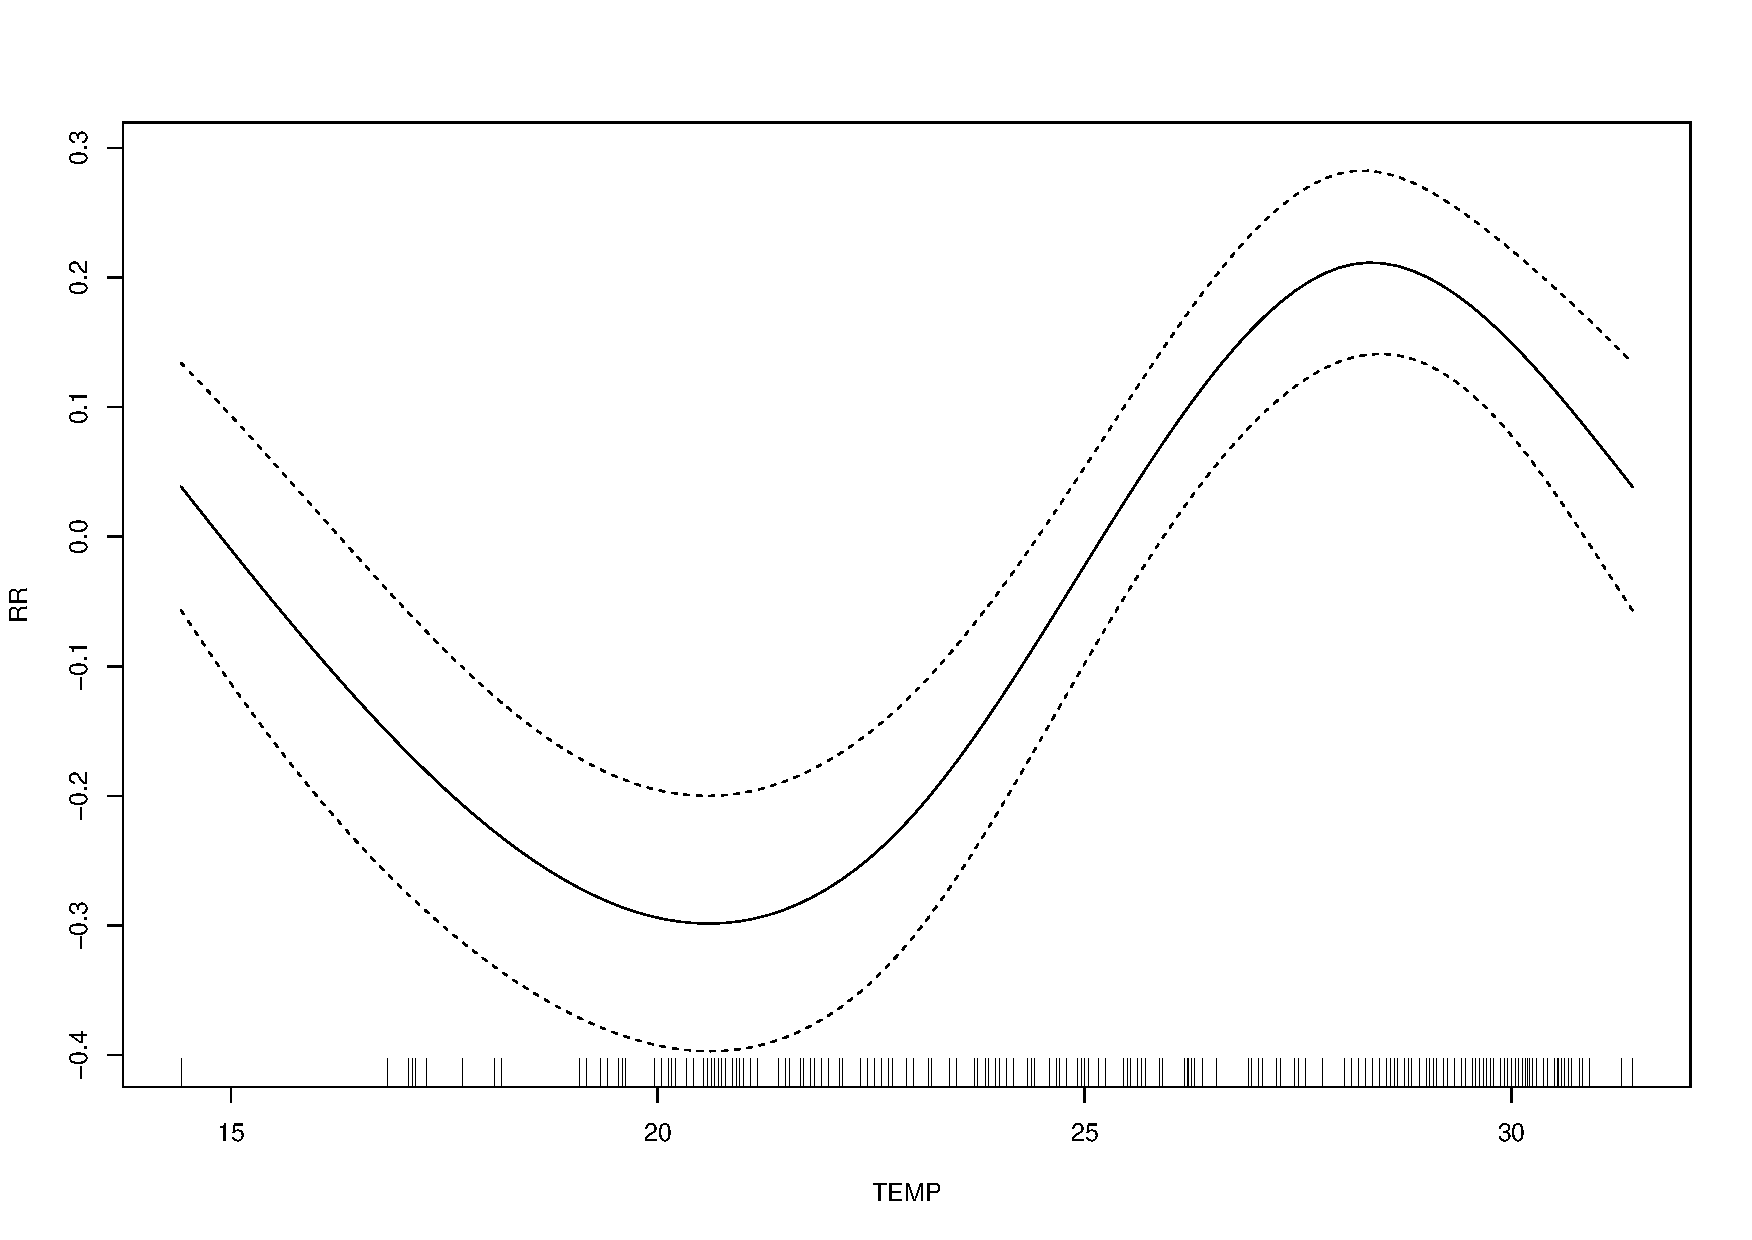
\includegraphics[width=10cm]{TEMPSMOOTH}
      \caption{smoothing TEMP}
\end{figure}

\begin{figure}
       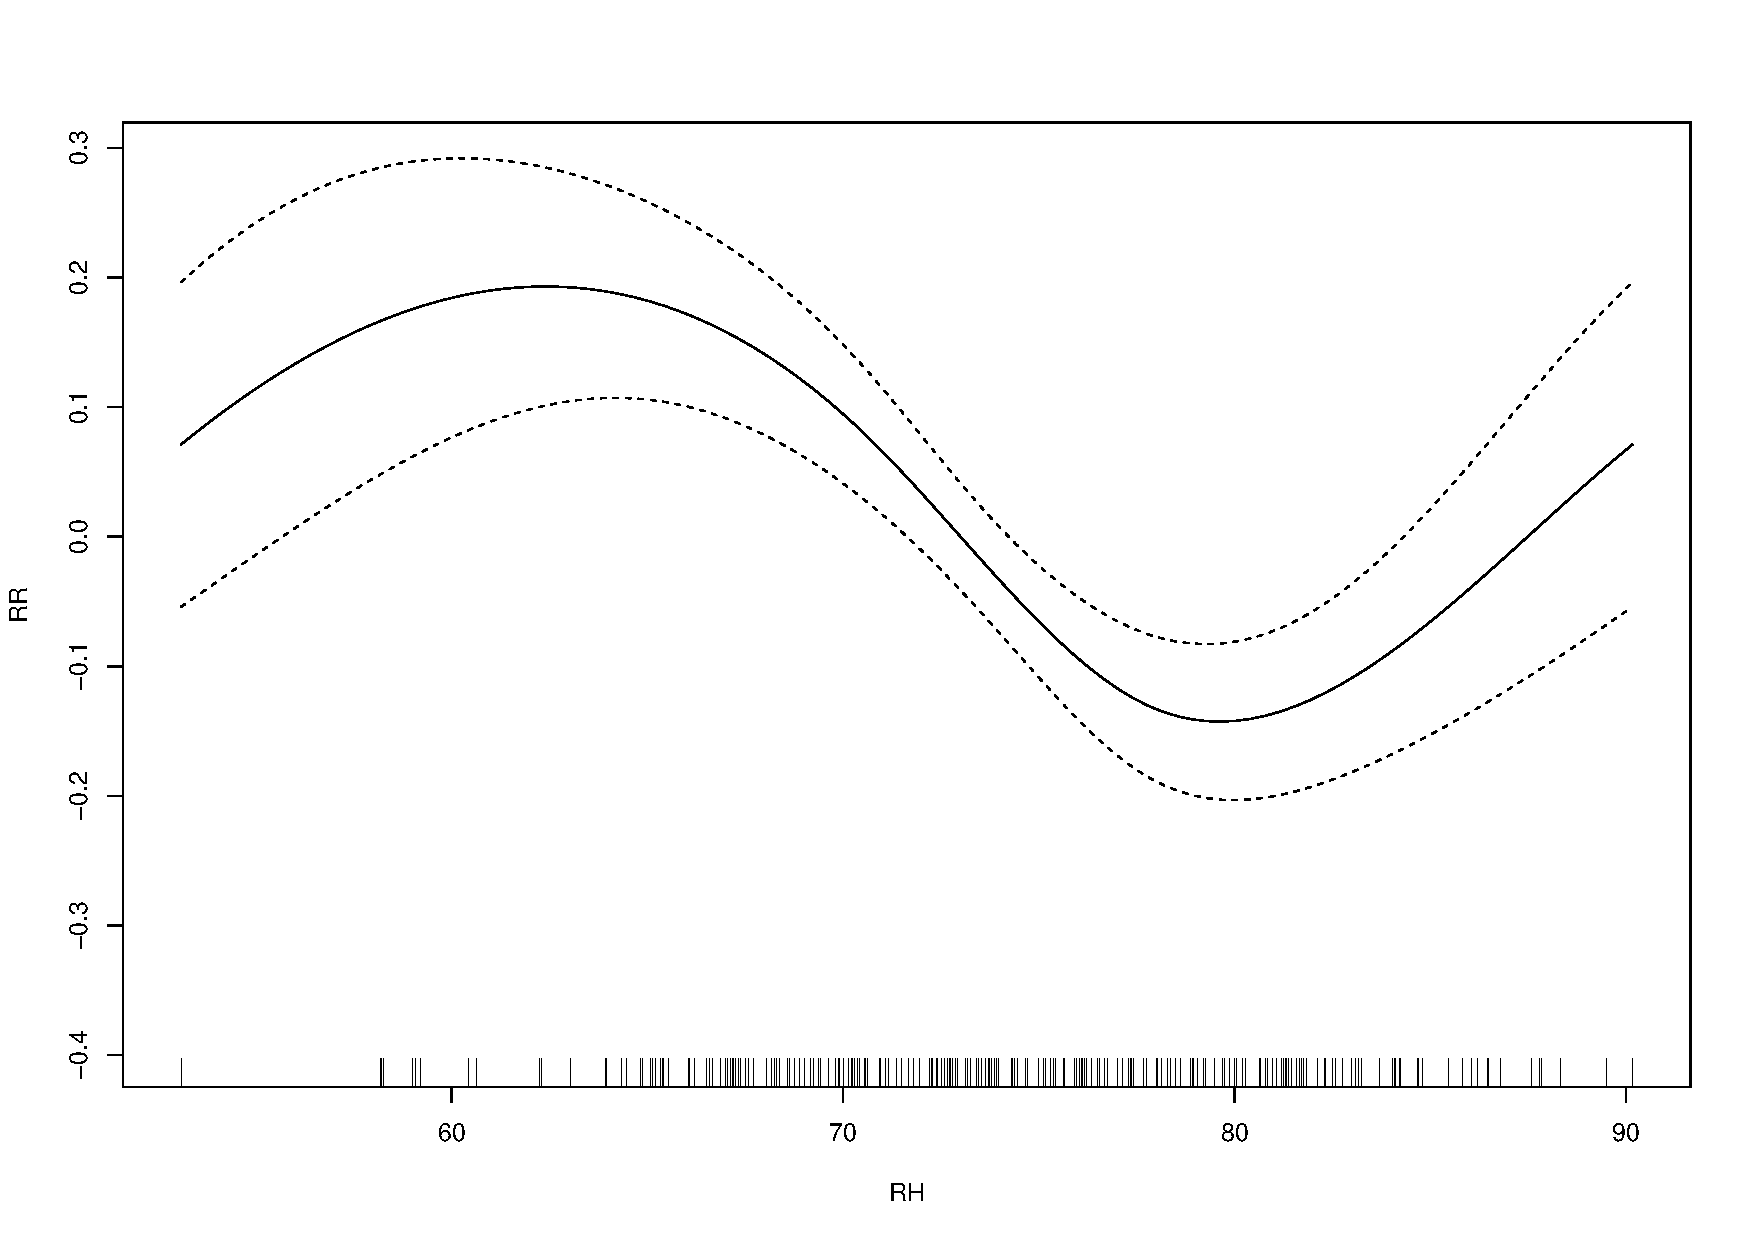
\includegraphics[width=10cm]{RHSMOOTH}
      \caption{smoothing RH}
\end{figure}


\end{document} 